\documentclass{article}
\usepackage[top=1in, bottom=1in, left=1in, right=1in]{geometry}
\usepackage{amsmath}
\usepackage{graphicx}
\begin{document}

\begin{flushright}
Matt Jibson \\
ST 521 \\
HW 3
\end{flushright}

\begin{enumerate}
	\item %1
		\begin{displaymath}
			P^n = \left( \begin{array}{ccc} 1 & 0 & 0 \\ (1/4)^n & (1/2)^n & (1/4)^n \\ (3/4)^n & 0 & (1/4)^n \end{array} \right)
		\end{displaymath}
	\item %2
		\begin{enumerate}
			\item
				$U_{10} = P_{10} + P_{11} U_{10} + P_{12} U_{20} \\
				U_{20} = P_{20} + P_{21} U_{10} + P_{22} U_{20} \\$
				or \\
				$U_{10} = 0.1 + 0.6 U_{10} + 0.1 U_{20} \\
				U_{20} = 0.2 + 0.3 U_{10} + 0.4 U_{20} \\$
				so \\
				$U_{10} = 8/21, U_{20} = 11/21$
			\item
				$\nu_1 = 1 + .6 \nu_1 + .1 \nu_2 \\
				\nu_2 = 1 + .3 \nu_1 + .4 \nu_2$ \\
				\begin{displaymath}
					\left( \begin{array}{cc} .4 & -.1 \\ -.3 & .6 \end{array} \right)
					\left( \begin{array}{c} \nu_1 \\ \nu_2 \end{array} \right) =
					\left( \begin{array}{c} 1 \\ 1 \end{array} \right) \Rightarrow
					\nu_1 = \nu_2 = 10/3
				\end{displaymath}
		\end{enumerate}
	\item %3
		%$U_i = p U_{i+1} + q U_i, i = 0, 1, 2, 3, \\
		%U_4 = 1 \\$
		$\nu_i = 1 + p \nu_{i+1} + q \nu_0, i = 0, 1, 2, 3 \\
		\nu_4 = 0$ \\
		$\nu_0 = 1 + q \nu_0 + p (1 + q \nu_0 + p (1 + q \nu_0 + p (1 + q \nu_0 + p (\nu_4)))) = \\
		1 + q \nu_0 + p + p q \nu_0 + p^2 + p^2 q \nu_0 + p^3 + p^3 q \nu_0 =
		1 + q \nu_0 + p (1 + q \nu_0) + p^2 (1 + q \nu_0) + p^3 (1 + q \nu_0) = \\
		(1 + q \nu_0) (1 + p + p^2 + p^3) = \nu_0$
		%Since $1 - p = q$, $\nu_i = 1 + q \nu_0 + p \nu_{i+1} \Rightarrow p \nu_i = 1 + p \nu_{i+1}, i = 0, 1, 2, 3$ \\
		%$\nu_0 = 1 + q \nu_0 + (1 + p \nu_1) = 1 + q \nu_0 + (1 + (1 + p \nu_2)) = 1 + q \nu_0 + (1 + (1 + (1 + p \nu_3))) = 1 + q \nu_0 + (1 + (1 + (1 + (1 + p \nu_4)))) = 1 + q \nu_0 + 4 = 5 + q \nu_0$
		%Look for a solution of the form $\nu_i = \Theta^i$, which gives $\Theta^i = 1 + p \Theta^{i+1} + q \Theta^{0}$. If $\Theta \ne 0$ then $\Theta = p \Theta^2 + q$.
	\item %4
		Probability $P_n$ of having $n$ boys: \\
		$P_0 = 1/4 + (3/4 * 1/8) = 11/32, P_1 = (3/4 * 3/8) = 9/32, P_2 = 9/32, P_3 = (3/4 * 1/8) = 3/32$ \\
		$\mu = 9/32 + 2 * 9/32 + 3 * 3/32 = 36/32 > 1$. \\
		$\phi(s) = 11/32 + 9/32 s + 9/32 s^2 + 3/32 s^3, \phi'(1) = \mu$, so the probability of ultimate extinction is \\
		$\frac{11}{32} + \frac{9 t}{32} + \frac{9 t^2}{32} + \frac{3 t^3}{32} = t \Rightarrow 32 (11 + 9t + 9t^2 + 3t^3) = 0$, which has solutions at $t = 2.38672, 0.306639 \pm 1.20094i$. But $\phi(s)$ is not convex, so does this analysis hold?
	\item %5
		$p_k = (1 - c) c^k, 0 < c < 1, k = 0, 1, \dots$. \\
		$\phi(t) = (1 - c) \Sigma_{k=1}^\infty c^{k-1} t^k = (1 - c) \frac{t}{1 - ct}, \mu = |\phi'(1)| = \frac{1 - c}{(1 - c)^2} = \frac{1}{1 - c} > 1$. \\
		$(1 - c) \frac{t}{1 - ct} = t \Rightarrow (1 - c) t = t - ct^2 \Rightarrow -ct + ct^2 = 0 = c (t^2 - t) = ct(t - 1) \Rightarrow \eta = 0$
	\item %6
		$p'(1) = .05 + 2 * .03 + 3 * .07 + 4 * .4 + 5 * .25 + 6 * .05 = 3.47 > 1$. \\
		$.15 - .95t + .03t^2 + .07t^3 + .4t^4 + .25t^5 + .05t^6 = 0 \Rightarrow \eta = 0.1592928$
	\item %7
		If $|\phi'(1)| = 2a + b < 1, \eta = 1$. If $|\phi'(1)| > 1,
		\eta$ is the smallest nonnegative value of $\frac{-b \pm \sqrt{b^2 - 4ac}}{2a}$ that is $< 1$.
	\item %8
		\begin{enumerate}
			\item For $\mu \le 1$ extinction occurs with probability 1, so $W$ is finite.
			\item $E(W_n) = \Sigma_{k=0}^n \mu^k$. If $\mu \ge 1$ then as $n \rightarrow \infty, E(W_n) \rightarrow \infty$. If $\mu < 1$ then as $n \rightarrow \infty, E(W_n) \rightarrow \frac{1}{1 - \mu}$.
		\end{enumerate}
	\newpage
	\item %9
		\ \\
		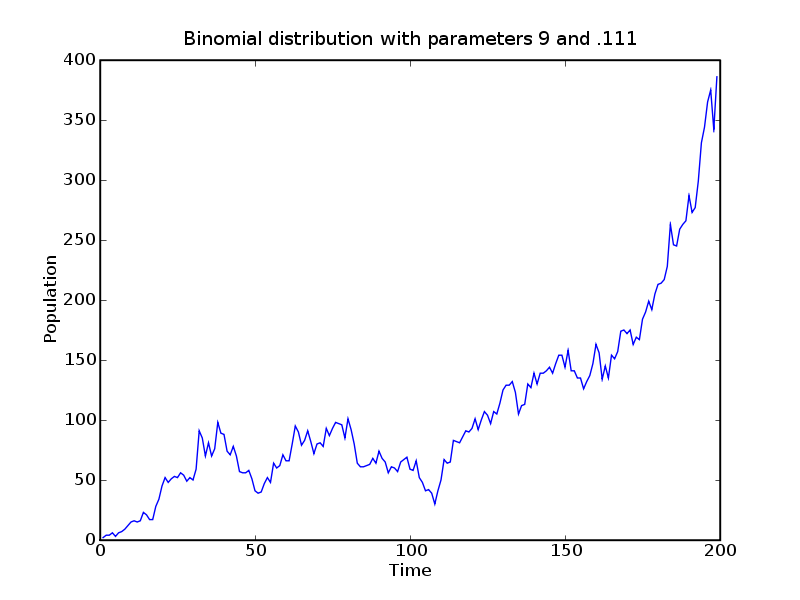
\includegraphics[width=0.7\linewidth]{binom} \\
		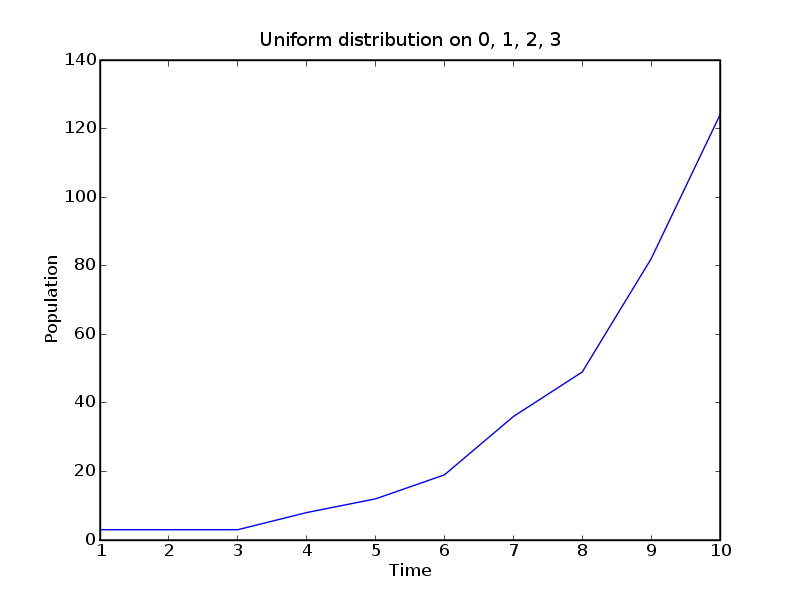
\includegraphics[width=0.7\linewidth]{uniform} \\
		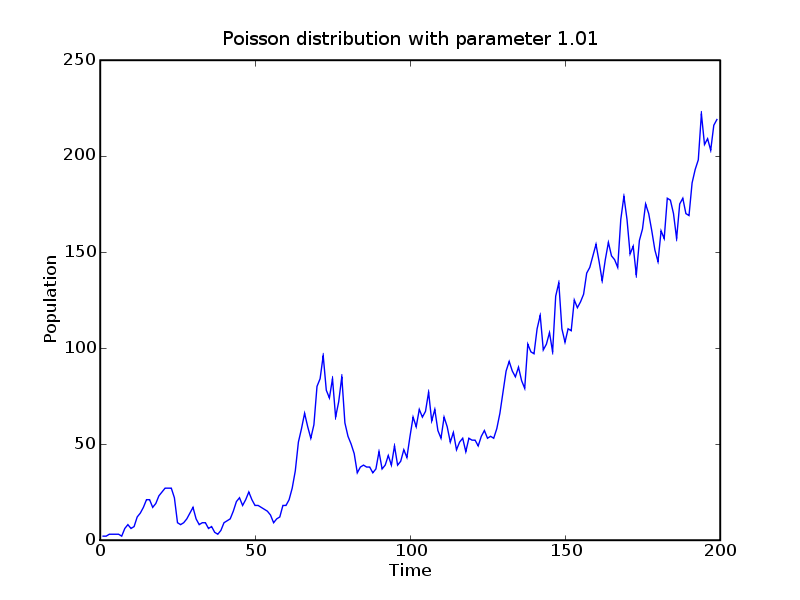
\includegraphics[width=0.7\linewidth]{poisson} \\
		Generated by some python (with appropriate changes for uniform and poisson):
		{\tiny
		\begin{verbatim}
from pylab import *
from random import *

def fac(n):
    if n <= 1:
        return 1
    else:
        return n * fac(n - 1)

def comb(n, k):
    return fac(n) / (fac(k) * fac(n - k))

def bernoulli(k, n, p):
    return comb(n, k) * p ** k * (1. - p) ** (n - k)

def poisson(k, l):
    return exp(-l) * l**k / fac(k)

prob = []

n = 9
p = .111
tot = 0
for i in range(n + 1):
    tot += bernoulli(i, n, p)
    prob.append(tot)

while True:
    t = []
    prev = 1
    s = range(1, 200)

    for i in s:
        cur = 0
        for j in range(prev):
            r = random()
            for k in range(len(prob)):
                if r < prob[k]:
                    cur += k
                    break

        t.append(cur)
        prev = cur

    if cur == 0:
        continue

    plot(s, t)
    xlabel('Time')
    ylabel('Population')
    title('Binomial distribution with parameters 9 and .111')
    savefig('binom')
    show()
    break
		\end{verbatim}
		}
\end{enumerate}

\end{document}